\section{实验设计与评价规约}\label{sec:protocol}

\subsection{评价对象与操作性定义}\label{sec:estimands}\label{sec:rq}

令
\[
 \theta=(g,\rho,s,r,\varphi,\mathcal C)
\]
表示一个完整的零假设条件，其中 $g$ 为数据生成过程，$\rho$ 为原序列依赖参数，$s$ 为窗口步长，$r\in\{\mathrm{fixed}\text{-}M,\mathrm{fixed}\text{-}T\}$ 为预算制度，$\varphi\in\{\mathrm{BPI},\mathrm{MOMENTS}\}$ 为表示，$\mathcal C\in\{\mathrm{M0},\mathrm{M1}\}$ 为校准方法。名义显著性水平固定为 $\alpha=0.05$，条件化有效尺寸定义为
\begin{equation}\label{eq:effective-size}
 \alpha_{\mathrm{eff}}(\theta)
 =\Pr_{H_0,\theta}\{p_\theta\le0.05\}.
\end{equation}
映射 $\theta\mapsto\alpha_{\mathrm{eff}}(\theta)$ 构成本文的有限样本校准表面。本文所称经验校准边界，是预设设计网格中逐格有效尺寸由实用校准区转入保守区或反保守区时形成的条件边界。

每个零假设配置均报告拒绝率及无连续性修正的 Wilson 区间。预先冻结的实用等价带为
\[
 \mathcal E=[0.035,0.065].
\]
逐格分类规则如下：90\% Wilson 区间完整包含于 $\mathcal E$ 时，记为点态实用校准；95\% Wilson 区间上界低于 $0.035$ 时，记为实质保守；95\% Wilson 区间下界高于 $0.065$ 时，记为实质反保守；其余情形记为边界或未定。该分类属于点态判断，不构成设计域上的同时概率保证。

备择实验考察两个相互关联的对象：其一，使用匹配零假设经验临界值计算的尺寸标准化功效，用于比较表示所保留的信号信息；其二，基于观测扫描曲线得到的定位误差和“检出且定位成功”的联合概率。相应定义见第~\ref{sec:alternatives} 节和第~\ref{sec:h1-localization} 节。

\subsection{零假设数据生成过程}\label{sec:dgp}

首先生成平稳高斯 AR(1) 过程
\begin{equation}\label{eq:latent-ar}
 G_t=\rho G_{t-1}+\sqrt{1-\rho^2}\,\varepsilon_t,
 \qquad
 G_0\sim N(0,1),\quad
 \varepsilon_t\overset{\mathrm{iid}}{\sim}N(0,1),
\end{equation}
其中 $G_0$ 与全部新息相互独立，$\rho\in\{0,0.8\}$。实现中舍弃最初 1000 个值；由于初值取自平稳分布，该步骤作为统一的生成约定保留。

N-AR 直接取标量观测
\begin{equation}\label{eq:n-ar}
 X_t=G_t.
\end{equation}
N-CIRCLE 先以标准正态分布函数 $\Phi$ 作概率积分变换，再映射到单位圆：
\begin{equation}\label{eq:n-circle}
 U_t=\Phi(G_t),\qquad
 C(u)=(\cos 2\pi u,\sin 2\pi u),\qquad
 X_t=C(U_t)+0.08\eta_t,
\end{equation}
其中 $\eta_t\overset{\mathrm{iid}}{\sim}N_2(0,I_2)$，并与潜变量过程独立。对每个固定 $t$，$U_t$ 服从 $U(0,1)$；当 $\rho=0$ 时，两类原始过程均为独立同分布序列，当 $\rho=0.8$ 时则保留时间依赖。N-CIRCLE 的定义基于平稳高斯过程的边际变换，不涉及随机游走或增量过程。

\subsection{双预算制度}\label{sec:budget}

窗口宽度固定为 $W=64$，步长取
\[
 s\in\{8,16,32,64\}.
\]
本文采用两种互补的预算制度：
\begin{itemize}
\item \textbf{固定窗口数（fixed-$M$）}：令 $M=192$，并由 $T=W+s(M-1)$ 确定原始序列长度；对应的 $T$ 依次为 $1592$、$3120$、$6176$ 和 $12288$。
\item \textbf{固定观测长度（fixed-$T$）}：令 $T=3120$，并由式\eqref{eq:windows}确定窗口数；对应的 $M$ 依次为 $383$、$192$、$96$ 和 $48$。
\end{itemize}
固定窗口数制度保持扫描器接收的特征数量不变，固定观测长度制度保持原始数据预算不变。两种制度在 $s=16$ 时共享相同的 $(T,M)=(3120,192)$ 几何配置；共享配置按同一逻辑实验单元计数。因此，$2$ 个数据生成过程、$2$ 个依赖水平和两种预算制度最终形成 28 个唯一零假设配置。

表~\ref{tab:design}给出两种预算制度下的完整窗口几何。该表同时说明：7 个唯一窗口几何的来源；两种制度在 $s=16$ 处的共享；$T$ 与 $M$ 如何随制度和步长变化；以及 M1 依赖乘子带宽为何随配置改变。

\begin{table}[ht]
\centering
\caption{双预算制度下的窗口几何设计。重叠率为 $1-s/W$；$b$ 为 M1 依赖乘子带宽，按 $b=\max\{\lfloor W/s\rfloor+1,\lceil M^{1/3}\rceil\}$ 确定。}\label{tab:design}
\begin{tabular}{cccccccc}
\toprule
$s$ & 重叠率 & \multicolumn{3}{c}{固定窗口数（fixed-$M$）} & \multicolumn{3}{c}{固定观测长度（fixed-$T$）}\\
\cmidrule(lr){3-5}\cmidrule(lr){6-8}
 & $1-s/W$ & $T$ & $M$ & $b$ & $T$ & $M$ & $b$\\
\midrule
8 & 87.5\% & 1592 & 192 & 9 & 3120 & 383 & 9\\
16 & 75.0\% & 3120 & 192 & 6 & 3120 & 192 & 6\\
32 & 50.0\% & 6176 & 192 & 6 & 3120 & 96 & 5\\
64 & 0\% & 12288 & 192 & 6 & 3120 & 48 & 4\\
\bottomrule
\end{tabular}

\begin{minipage}{0.94\textwidth}
\vspace{0.4em}
\footnotesize 注：$s=16$ 行在两种制度下给出相同的 $(T,M)=(3120,192)$，为共享配置；唯一配置计数中只计一次，但在两种预算视角下分别用于解释，因此该行会被两张热图有意重复展示。$s=64$ 时 $s=W$，窗口不重叠，重叠率为 0，对应 M1 保守性主对比 P3 的非重叠端。
\end{minipage}
\end{table}

图~\ref{fig:alternatives}展示两类备择构造的几何形态。

\begin{figure}[ht]
\centering
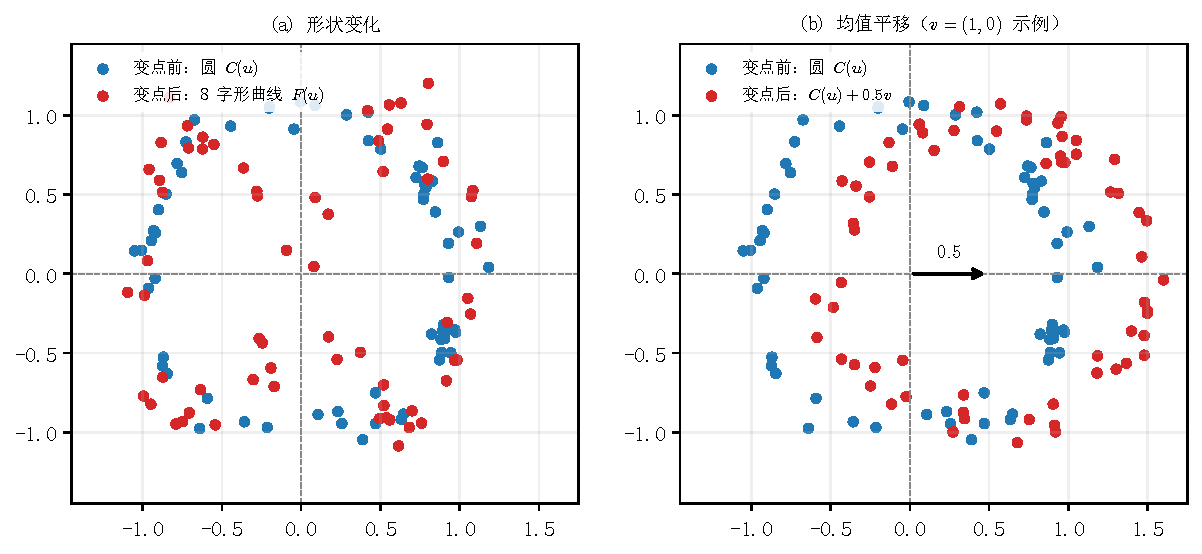
\includegraphics[width=0.95\textwidth]{../artifacts/figures/Figure2_alternative_geometry.pdf}
\caption{两类备择构造。左两幅为形状变化：变点前为圆形点云，变点后改为八字曲线；右两幅为均值平移：变点后圆形点云整体平移。圆与八字只匹配单时点均值与协方差，完整滞后联合分布未被声明为相同；平移备择直接改变均值。两个场景分别针对 BPI 与 MOMENTS 的结构敏感性。}\label{fig:alternatives}
\end{figure}

\subsection{Monte Carlo 设置}\label{sec:mc}

每个零假设配置独立复制 $R_0=2500$ 次，每个备择配置独立复制 $R_1=1600$ 次。每次方法校准均使用 $B=999$ 次内层重采样，并按式\eqref{eq:mc-pvalue}计算 $p$ 值。零假设部分包含
\[
 28\times2\text{（表示）}\times2\text{（方法）}\times2500
 =280{,}000
\]
条方法--表示评价记录；备择部分包含
\[
 2\text{（场景）}\times4\text{（条件）}\times2\text{（表示）}
 \times2\text{（方法）}\times1600
 =51{,}200
\]
条记录。外层 Monte Carlo 因而同时包含数据生成随机性与 $B=999$ 次内层校准的有限重采样随机性。

\subsection{预先设定的主对比}\label{sec:primary}

令 $\pi_{g,\rho,s,m}^{(r)}$ 表示在 BPI 表示、预算制度 $r$ 和校准方法 $m\in\{\mathrm{M0},\mathrm{M1}\}$ 下的零假设拒绝概率，且 $g\in\mathcal G=\{\mathrm{N\mbox{-}AR},\mathrm{N\mbox{-}CIRCLE}\}$。三个主对比均在确认性分析前冻结：
\begin{align}
\mathrm{P1}:\quad
 D_{\mathrm{OV}}^{M}
 &=\frac12\sum_{g\in\mathcal G}
 \left(\pi_{g,0,16,\mathrm{M0}}^{(M)}
      -\pi_{g,0,64,\mathrm{M0}}^{(M)}\right),
 \label{eq:p1}\\
\mathrm{P2}:\quad
 D_{\mathrm{ST}}^{T}
 &=\frac12\sum_{g\in\mathcal G}
 \left(\pi_{g,0,16,\mathrm{M0}}^{(T)}
      -\pi_{g,0,64,\mathrm{M0}}^{(T)}\right),
 \label{eq:p2}\\
\mathrm{P3}:\quad
 D_{\mathrm{CONS}}
 &=0.05-\frac12\sum_{g\in\mathcal G}
 \pi_{g,0,64,\mathrm{M1}}^{(M)}.
 \label{eq:p3}
\end{align}
P1 与 P2 检验单侧假设 $D\le0.10$ 对 $D>0.10$；P3 检验 $D_{\mathrm{CONS}}\le0.01$ 对 $D_{\mathrm{CONS}}>0.01$。MOMENTS 的同构对比仅作次级描述，不进入主要多重性族。

主对比使用 10,000 次按数据生成过程分层的整簇自助法。同一主重复编号下的全部相关条件、表示和方法随簇共同重采样，以保留配对结构。对一般效应量 $\widehat\theta$ 及单侧阈值 $\theta_0$，自助 $p$ 值定义为
\begin{equation}\label{eq:bootstrap-p}
 p_{\mathrm{boot}}
 =\frac{1+\sum_{b=1}^{10000}
 \mathbf1\{\widehat\theta_b^*-\widehat\theta
 \ge \widehat\theta-\theta_0\}}
 {10001}.
\end{equation}
因此，自助 $p$ 值不可能等于零。若 $q_\gamma$ 表示 10,000 个自助估计的 nearest-rank $\gamma$ 分位数，则边际 95\% basic 区间为
\begin{equation}\label{eq:basic-ci}
 \left[2\widehat\theta-q_{0.975},\,
       2\widehat\theta-q_{0.025}\right],
 \qquad
 q_\gamma=\widehat\theta^*_{(\lceil10000\gamma\rceil)}.
\end{equation}
三个单侧 $p$ 值采用 Holm step-down 校正，族水平为 $0.05$。本文将校正后 $p\le0.05$ 作为预先设定的操作性支持标准，同时用式\eqref{eq:basic-ci}报告效应量不确定性；该区间为边际区间，不解释为 Holm 同时置信区间。

\subsection{备择构造与尺寸标准化功效}\label{sec:alternatives}

备择实验以 N-CIRCLE 为基础，并在完整序列上连续生成同一潜变量过程和观测噪声，不在变点处重置随机状态。令
\[
 \tau=\left\lfloor\frac T2\right\rfloor,
 \qquad
 F(u)=(\sin2\pi u,\sin4\pi u).
\]
形状变化场景定义为
\begin{equation}\label{eq:shape-alt}
 X_t=
 \begin{cases}
 C(U_t)+0.08\eta_t, & t\le\tau,\\
 F(U_t)+0.08\eta_t, & t>\tau.
 \end{cases}
\end{equation}
当 $U_t\sim U(0,1)$ 时，$C(U_t)$ 与 $F(U_t)$ 的单时点均值均为零，协方差均为 $I_2/2$；加入同分布噪声后，这两个单时点边际矩仍保持匹配。该构造不要求变点前后的完整滞后联合分布或二阶过程相同。

均值平移场景定义为
\begin{equation}\label{eq:mean-alt}
 X_t=C(U_t)+0.08\eta_t+0.5v\mathbf1\{t>\tau\},
 \qquad
 v=(\cos2\pi V,\sin2\pi V),\quad V\sim U(0,1),
\end{equation}
其中每次 Monte Carlo 重复抽取一个方向 $v$，并在该重复内固定。每个备择场景均使用 $M=192$、$s\in\{16,64\}$ 和 $\rho\in\{0,0.8\}$，共四个条件。

尺寸标准化功效使用与备择条件、表示和几何配置匹配的零假设观测统计量。将 $R_0=2500$ 个零假设统计量按升序记为
\[
 T_{M,(1)}^{H_0}\le\cdots\le T_{M,(R_0)}^{H_0},
\]
并令
\begin{equation}\label{eq:h0-critical}
 j_{0.95}=\left\lceil0.95(R_0+1)\right\rceil=2376,
 \qquad
 \widehat c_{0.95}^{H_0}=T_{M,(2376)}^{H_0}.
\end{equation}
对备择统计量 $T_{M,r}^{H_1}$，定义
\begin{equation}\label{eq:size-standardized-power}
 \widehat\beta_{\mathrm{std}}
 =\frac1{R_1}\sum_{r=1}^{R_1}
 \mathbf1\{T_{M,r}^{H_1}>\widehat c_{0.95}^{H_0}\}.
\end{equation}
由于 M0 与 M1 共享同一观测统计量，式\eqref{eq:size-standardized-power}在每个“条件--表示”组合上只计算一次，用于评价表示敏感性，不用于排列两种校准方法的优劣。

\subsection{可复现性边界}\label{sec:repro}

实验协议、随机种子、配置和主要分析规则均在确认性分析前冻结。零假设与备择结果来自不可变的正式试次记录，正文数值由统一汇总文件生成。试次身份、配置哈希、环境锁定、失败留证和完整逐格结果在补充材料及代码仓库中提供；这些工程记录服务于结果追溯，不构成本文的独立方法贡献。
